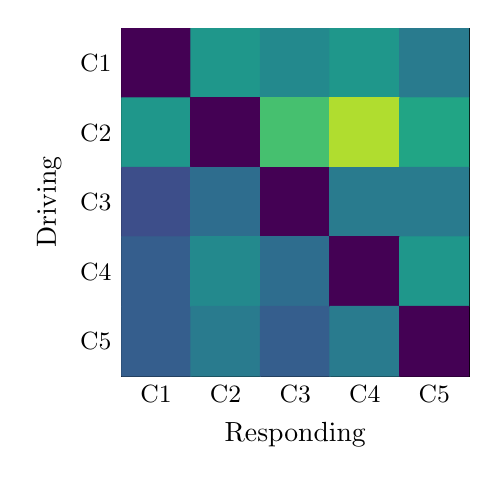
\begin{tikzpicture}
\begin{axis}[
    xlabel={Responding},
    ylabel={Driving},
    xtick={1,2,3,4,5},
    ytick={1,2,3,4,5},
    xticklabels={C1, C2, C3, C4, C5},
    yticklabels={C1, C2, C3, C4, C5},
    colormap/viridis,
    % colormap name=coolwarm,
    % colorbar,
    % colorbar style={
    % ytick={0,0.05,0.10,0.15},
    % yticklabels={0.00, 0.05, 0.10, 0.15},
    % width=0.4cm,
    % },
    point meta min=0,
    point meta max=0.17,
    enlargelimits=false,
    tick label style={font=\small},
    width=6cm,
    height=6cm,
    y dir=reverse,
]
\addplot[
    matrix plot*,
    mesh/cols=5,
    point meta=explicit,
] table [meta=C] {
x y C
1 1 0.00
2 1 0.09
3 1 0.08
4 1 0.09
5 1 0.07
1 2 0.09
2 2 0.00
3 2 0.12
4 2 0.15
5 2 0.10
1 3 0.04
2 3 0.06
3 3 0.00
4 3 0.07
5 3 0.07
1 4 0.05
2 4 0.08
3 4 0.06
4 4 0.00
5 4 0.09
1 5 0.05
2 5 0.07
3 5 0.05
4 5 0.07
5 5 0.00
};
\end{axis}
\end{tikzpicture}
